\documentclass[11pt]{article}
\usepackage[margin=2.5cm]{geometry}
\usepackage{listings}
\usepackage{xcolor}
\usepackage{hyperref}
\usepackage{booktabs}
\usepackage{parskip}
\usepackage{enumitem}
\usepackage{graphicx}
\usepackage{float}
\usepackage{caption}

\definecolor{codebg}{RGB}{245,246,248}
\lstset{
  basicstyle=\ttfamily\small,
  backgroundcolor=\color{codebg},
  frame=single,
  numbers=left,
  numberstyle=\tiny,
  breaklines=true,
  showstringspaces=false,
  columns=fullflexible,
  keywordstyle=\bfseries,
}
\captionsetup{font=small,labelfont=bf}

\title{MRN Project 1: PHY/MAC Metrics Collection xApp}
\author{Giorgio Messina \\ \texttt{giorgio.messina@mail.polimi.it}}
\date{}

\begin{document}
\maketitle
\vspace{-1.5cm}

\section{Overview}
This report describes a Proof of Concept xApp for O-RAN that collects PHY and MAC layer metrics from a gNB emulator (gNBemu) through a custom, non 3GPP E2 Service Model carried over UDP with Protocol Buffers instead of ASN.1. The system has three parts: a protobuf schema shared by both endpoints, a Python xApp running against the near-RT RIC, and a C message handler on the gNB emulator side. Every 500 ms the xApp requests the RSRP, uplink and downlink BER, and uplink and downlink MCS of every connected UE, together with the current cell load (allocated PRBs against the maximum), and appends everything with a timestamp to two CSV files. I also wrote a small script to visualize the collected data, described in Section 5.

\section{Protocol design}
The schema follows the official Protocol Buffers style guide: CamelCase names for messages and enums (\texttt{RanMessage}, \texttt{UeInfo}, \texttt{UeList}, \texttt{RanParameterMapEntry}, ...), which maps predictably onto both the generated Python classes and, on the C side, the protobuf-c generated structs (\texttt{RanMessage} becomes \texttt{ran\_message\_\_pack}, \texttt{UeList} becomes \texttt{ue\_list\_\_init}, and so on).

\begin{lstlisting}[language=C]
enum RanParameterId {
  GNB_ID           = 1;
  UE_LIST          = 3;
  GLOBAL_PRB_ALLOC = 5;
  MAX_PRB          = 6;
}
message UeInfo {
  required uint32 rnti = 1;
  optional float rsrp_dbm = 2;
  optional float ber_ul = 3;
  optional float ber_dl = 4;
  optional uint32 mcs_ul = 5;
  optional uint32 mcs_dl = 6;
}
\end{lstlisting}

\texttt{rnti}, \texttt{mcs\_ul}, \texttt{mcs\_dl} and \texttt{connected\_ues} are \texttt{uint32}, since none of them can be negative. I left a few enum values and field numbers explicitly \texttt{reserved} for parameters I might add later (an extra cell or slice identifier, an additional measurement), so the numbering stays stable if the schema grows. \texttt{UeInfo} also carries two generic fields, \texttt{aux\_flag} and \texttt{aux\_value}, meant for control-oriented variants of this xApp (for example forcing a lower MCS or limiting the PRBs assigned to a UE) that are not exercised by this metrics-collection version.

\section{gNB emulator}
The emulator keeps a fixed-size fleet of simulated UEs and answers indication requests from the xApp with randomly generated but signal-consistent measurements. RSRP is sampled uniformly between $-65$ and $-109$ dBm (representative of an N78 deployment), and BER/MCS are then drawn from one of three bands depending on that RSRP value, since a UE with a strong signal should not realistically report a bad BER or a low MCS.

\begin{center}
\small
\begin{tabular}{lccc}
\toprule
RSRP range & BER DL & BER UL & MCS range \\
\midrule
$\geq -80$ dBm & 0.000 to 0.004 & DL + 0.001 to 0.005 & 20 to 27 (256-QAM) \\
$-95$ to $-80$ dBm & 0.000 to 0.049 & DL + 0.005 to 0.025 & 10 to 19 (64-QAM) \\
$< -95$ dBm & 0.000 to 0.199 & DL + 0.010 to 0.059 (cap 0.3) & 0 to 9 (QPSK/16-QAM) \\
\bottomrule
\end{tabular}
\end{center}

All the mutable state of the emulator (gNB id, PRB counters, initialization flag, the simulated UE array) is grouped into a single struct instead of being spread across file-scope globals, and the RSRP-to-BER/MCS logic above is split into three small functions (\texttt{classify\_link\_quality}, \texttt{sample\_ber}, \texttt{sample\_mcs}) instead of being inlined inside the function that builds the UE list:

\begin{lstlisting}[language=C]
static void sample_ber(link_quality_t quality, float *ber_ul, float *ber_dl) {
  switch (quality) {
    case LINK_QUALITY_STRONG:
      *ber_dl = (rand() % 5) / 1000.0f;
      *ber_ul = *ber_dl + 0.001f + (rand() % 5) / 1000.0f;
      break;
    case LINK_QUALITY_MEDIUM:
      *ber_dl = (rand() % 50) / 1000.0f;
      *ber_ul = *ber_dl + 0.005f + (rand() % 20) / 1000.0f;
      break;
    case LINK_QUALITY_WEAK:
    default:
      *ber_dl = (rand() % 200) / 1000.0f;
      *ber_ul = *ber_dl + 0.01f + (rand() % 50) / 1000.0f;
      break;
  }
  if (*ber_ul > BER_UL_CAP) *ber_ul = BER_UL_CAP;
}
\end{lstlisting}

Unrecognized or unimplemented message types are logged and dropped rather than triggering an \texttt{assert()}, since a component meant to run unattended should not abort just because it received something unexpected. The function that frees a UE list also sets every pointer to \texttt{NULL} right after freeing it, to avoid ever touching a freed pointer by mistake. Parameter ids are also mapped to a short name for the log lines, in the same spirit as the enum itself:

\begin{lstlisting}[language=C]
static const char *ran_parameter_name(RanParameterId param_id) {
  switch (param_id) {
    case RAN_PARAMETER_ID__GNB_ID:           return "gnb_id";
    case RAN_PARAMETER_ID__UE_LIST:          return "ue_list";
    case RAN_PARAMETER_ID__GLOBAL_PRB_ALLOC: return "global_prb_alloc";
    case RAN_PARAMETER_ID__MAX_PRB:          return "max_prb";
    default:                                 return "unrecognized_param";
  }
}
\end{lstlisting}

Figure~\ref{fig:ber} shows the BER reported over a short test run against RSRP: the three sampling bands from the table above are clearly visible.

\begin{figure}[H]
  \centering
  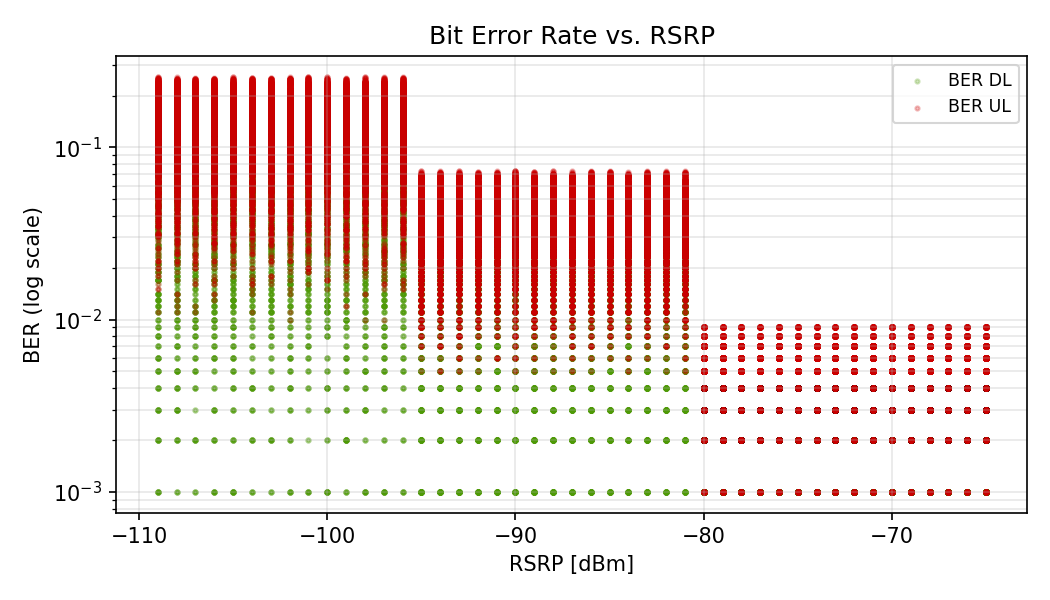
\includegraphics[width=0.72\textwidth]{fig_ber_vs_rsrp.png}
  \caption{Downlink and uplink BER against RSRP. The three tiers used to sample BER and MCS appear as separate bands.}
  \label{fig:ber}
\end{figure}

\section{xApp}
The xApp is organized into a few independent pieces instead of one large function: a small dataclass for the configuration (poll interval, output paths, requested parameters), a class that owns the two CSV files and knows how to append rows to them, a plain function that turns a decoded \texttt{RanIndicationResponse} into a small object with only the fields I need, and a class that ties discovery, subscription and the polling loop together. Keeping the parsing function independent of the RIC connection means it can be tested on its own, by building a fake response in memory, which is how I checked it behaves correctly without needing a live RIC:

\begin{lstlisting}[language=Python]
def parse_indication_response(response):
    snapshot = CellSnapshot()
    for entry in response.param_map:
        name = ransm.RanParameterId.Name(entry.key)
        if name == "GNB_ID" and entry.HasField("string_value"):
            snapshot.gnb_id = entry.string_value
        elif name == "MAX_PRB":
            snapshot.max_prb = entry.int64_value
        elif name == "GLOBAL_PRB_ALLOC":
            snapshot.allocated_prb = entry.int64_value
        elif name == "UE_LIST":
            snapshot.ue_list = list(entry.ue_list.ue_info)
    return snapshot
\end{lstlisting}

Logging uses the standard \texttt{logging} module instead of \texttt{print}, and the poll interval and output folder are command line arguments (\texttt{--poll-interval}, \texttt{--out-dir}), defaulting to the 500 ms interval used throughout the project.

The two CSV files are:
\begin{lstlisting}
e2sm_data.csv:   timestamp, gnb_id, allocated_prb, max_prb, load
e2smue_data.csv: timestamp, gnb_id, rnti, rsrp_dbm, ber_ul, ber_dl, mcs_ul, mcs_dl
\end{lstlisting}

\section{Data visualization}
Since the xApp only writes CSV files, I wrote \texttt{visualize\_ran\_metrics.py} (pandas and matplotlib) to make sense of the collected data without having to open a spreadsheet. It prints a short summary (sample counts, number of distinct UEs, average load, average BER and MCS) and produces a few plots: cell load over time, RSRP distribution, BER against RSRP, MCS distribution, and a combined dashboard with all four. Figure~\ref{fig:load} shows the cell load over a short run: allocated PRBs swing between nearly idle and fully loaded quite quickly, since each indication currently samples the load independently rather than following a smoother, more realistic traffic pattern.

\begin{figure}[H]
  \centering
  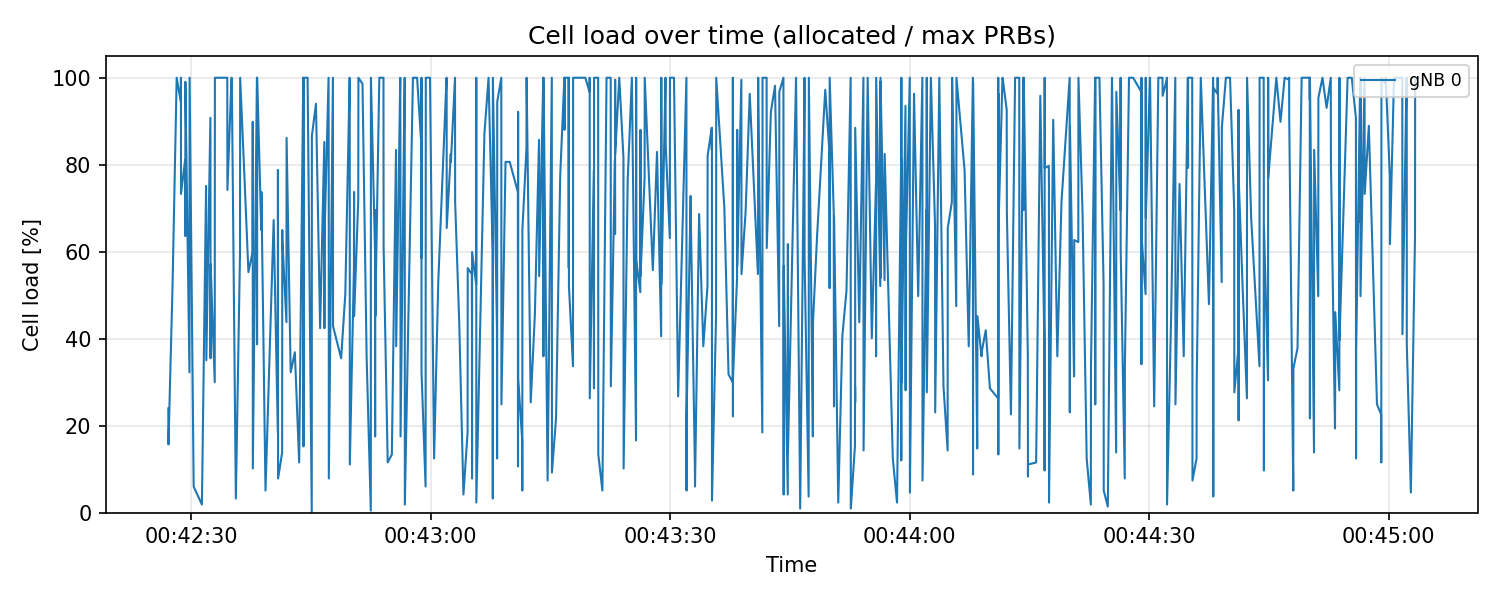
\includegraphics[width=0.72\textwidth]{fig_cell_load.png}
  \caption{Cell load (allocated PRBs over the maximum) during a short test run.}
  \label{fig:load}
\end{figure}

\section{Known limitations}
The gNB handler was checked with \texttt{gcc -fsyntax-only} against a header written to match protobuf-c's naming conventions, not against a header actually generated by \texttt{protoc-c}, since that toolchain was not available while preparing this report. Before relying on this for a live demo, the natural next step is to regenerate \texttt{ran\_messages.pb-c.h} with \texttt{protoc-c}, build the emulator against it, and run the full chain against a real near-RT RIC instance. The cell load and BER/MCS models are also independent random samples rather than derived from a shared SNR estimate, a more accurate version would compute BER from an estimated SNR and a link-adaptation table using the Q-function, which I left as a possible improvement.

\end{document}
